\section{Rozwiązanie VPN dla Pracowników Zdalnych}
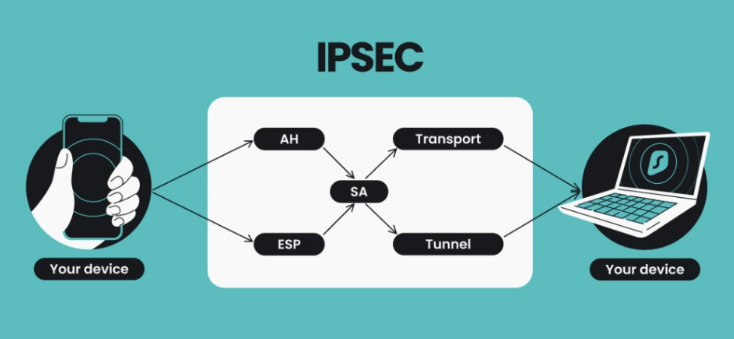
\includegraphics[width=0.8\textwidth]{vpn.png}

\subsection{Specyfikacja Techniczna Sprzętu VPN}

    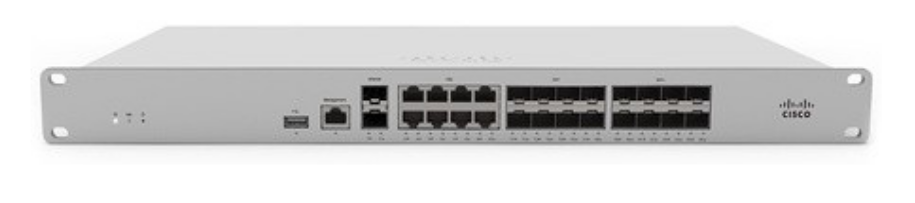
\includegraphics[width=0.6\textwidth]{3-vpn.png}

    \begin{flushleft}
        \begin{table}[h]
            \renewcommand{\arraystretch}{1.5}
            \begin{tabular}{|l|l|}
                \hline
                \textbf{Opis produktu} & Cisco Meraki MX450-HW Cloud Managed - firewall \\
                \hline
                \textbf{Rodzaj urządzenia} & Firewall \\
                \hline
                \textbf{Ilość Anten} & Brak \\
                \hline
                \textbf{Rodzaj obudowy} & Montowany w szafie rack 1U \\
                \hline
                \textbf{Interfejs} & 2 x SFP+ WAN, 8 x 10/100/1000 + 8 x SFP + 8 x SFP+ \\
                \hline
                \textbf{Przepustowość} & 6 Gbps \\
                \hline
                \textbf{Maksymalna liczba użytkowników} & 10,000 \\
                \hline
                \textbf{Liczba tuneli VPN} & 5,000 \\
                \hline
                \textbf{USB dla 3G/4G} & Tak \\
                \hline
                \textbf{Wymiary (szer./głęb./wys.)} & 48.3cm x 44.0cm x 4.4cm \\
                \hline
                \textbf{Waga} & 7.3kg \\
                \hline
            \end{tabular}
        \end{table}
    \end{flushleft}
\subsection{Kosztorys Implementacji Rozwiązania VPN}
    \begin{flushleft}
        \begin{table}[h]
            \renewcommand{\arraystretch}{1.5}
            \begin{tabular}{|l|l|}
                \hline
                \textbf{Nazwa} & \textbf{Cena (zł)} \\
                \hline
                Cisco Meraki MX450-HW Cloud Managed - firewall & 86 124,90 \\
                Cisco Meraki LIC-MX67-SEC-5YR-licencja & 7 049,0 \\
                \hline
                \textbf{Suma} & \textbf{93 173,9} \\
                \hline
            \end{tabular}
        \end{table}
    \end{flushleft}